 \documentclass[12pt]{exam}

% essential packages
\usepackage{fullpage} % margin formatting
\usepackage{enumitem} % configure enumerate and itemize
\usepackage{amsmath, amsfonts, amssymb, mathtools} % math symbols
\usepackage{xcolor, colortbl} % colors, including in tables
\usepackage{makecell} % thicker \Xhline in table
\usepackage{graphicx} % images, resizing

% sometimes needed packages
\usepackage{hyperref} % hyperlinks
% \hypersetup{colorlinks=true, urlcolor=blue}
% \usepackage{logicproof} % natural deduction
% \usepackage{tikz} % drawing graphs
% \usetikzlibrary{positioning}
% \usepackage{multicol}
% \usepackage{algpseudocode} % pseudocode

% paragraph formatting
\setlength{\parskip}{6pt}
\setlength{\parindent}{0cm}

% newline after Solution:
\renewcommand{\solutiontitle}{\noindent\textbf{Solution:}\par\noindent}

% less space before itemize/enumerate
\setlist{topsep=0pt}

% creates \filcl to grey out cells for groupwork grading
\newcommand{\filcl}{\cellcolor{gray!25}}

% creates \probnum to get the problem number
\newcounter{probnumcount}
\setcounter{probnumcount}{1}
\newcommand{\probnum}{\arabic{probnumcount}. \addtocounter{probnumcount}{1}}

% use roman numerals by default
\setlist[enumerate]{label={(\roman*)}}

% creates custom list environments for grading guidelines, question parts
\newlist{guidelines}{itemize}{1}
\setlist[guidelines]{label={}, left=0pt .. \parindent, nosep}
\newlist{gwguidelines}{enumerate}{1}
\setlist[gwguidelines]{label={(\roman*)}, nosep}
\newlist{qparts}{enumerate}{2}
\setlist[qparts]{label={(\alph*)}}
\newlist{qsubparts}{enumerate}{2}
\setlist[qsubparts]{label={(\roman*)}}
\newlist{stmts}{enumerate}{1}
\setlist[stmts]{label={(\roman*)}, nosep}
\newlist{pflist}{itemize}{4}
\setlist[pflist]{label={$\bullet$}, nosep}
\newlist{enumpflist}{enumerate}{4}
\setlist[enumpflist]{label={(\arabic*)}, nosep}

 \printanswers

\newcommand{\prevhwnum}{4}
\newcommand{\hwnum}{5}

\begin{document}
%%%%%%%%%%%%%%% TITLE PAGE %%%%%%%%%%%%%%%
\title{EECS 203: Discrete Mathematics\\
  Winter 2024\\
  Homework \hwnum{}}
\date{}
\author{}
\maketitle
\vspace{-50pt}
\begin{center}
  \huge Due \textbf{Thursday, Mar. 7th}, 10:00 pm\\
\Large No late homework accepted past midnight.\\
\vspace{10pt}
\large Number of Problems: $7+2$
\hspace{3cm}
Total Points: $100+30$
\end{center}
\vspace{25pt}
\begin{itemize}
    \item \textbf{Match your pages!} Your submission time is when you upload the file, so the time you take to match pages doesn't count against you.
    \item Submit this assignment (and any regrade requests later) on Gradescope. 
    \item Justify your answers and show your work (unless a question says otherwise).
    \item By submitting this homework, you agree that you are in compliance with the Engineering Honor Code and the Course Policies for 203, and that you are submitting your own work.
    \item Check the syllabus for full details.
\end{itemize}
\newpage
%%%%%%%%%%%%%%% TITLE PAGE %%%%%%%%%%%%%%% 

\section*{Individual Portion}

\subsection*{\probnum Easy as 3, 18, 93 [16 points]}

 Let $P(n)$ be the statement that $3 + 3 \cdot 5 + 3 \cdot 5^2 + ... + 3 \cdot 5^n = \frac{3 (5^{n+1} - 1)}{4}$. In this problem, we will prove using weak induction that $P(n)$ is true whenever $n$ is a non-negative integer.
\begin{parts}
    \item What is the statement $P(0)$? Complete the base case by showing that $P(0)$ is true.
    \item In the base case we prove $P(0)$; what do you need to prove in the inductive step?
    \item What is the inductive hypothesis for your proof?
    \item Complete the inductive step, indicating where you used the inductive hypothesis.
    
    \textit{Reminder:} You should prove this equation using a chain of equalities, starting on one side and transforming it into the other side.  You should \textbf{not} start with the equation you want to prove and transform both sides to be equal.
    \item Explain why this proof shows $P(n)$ is true for all non-negative integers $n$.
\end{parts}

\begin{solution}
\begin{parts}
    \item Plug $n = 0$ into both sides of equation to get $P(0): 3 \cdot 5^0 = \frac{3 (5^{0+1} - 1)}{4}$.
    
    \textbf{Base case:} $n = 0$
    
    Starting from the right-hand side,
    $$\frac{3 (5^{0+1} - 1)}{4} = \frac{3 (5 - 1)}{4} = 3 \cdot \frac{4}{4} = 3 = 3 \cdot 5^0.$$
    Therefore, $P(0)$ is true.
    \item We want to show that for all integers $k \geq 0,$ $P(k) \rightarrow P(k+1)$.
    \item The inductive hypothesis is $3 + 3 \cdot 5 + 3 \cdot 5^2 + \dots + 3 \cdot 5^k = \frac{3 (5^{k+1} - 1)}{4}$ for some non-negative integer $k$. I.e. we assume $P(k)$ for some $k\ge 0.$
    \item Assume $3 + 3 \cdot 5 + 3 \cdot 5^2 + ... + 3 \cdot 5^k = \frac{3 (5^{k+1} - 1)}{4}$ for some integer $k \geq 0$ (the I.H.). Then,
    \begin{align*}
        3 + 3 &\cdot 5 + 3 \cdot 5^2 + ... + 3 \cdot 5^{k+1} \\
        &= 3 + 3 \cdot 5 + 3 \cdot 5^2 + ... + 3 \cdot 5^k + 3 \cdot 5^{k+1}\\
        &= \frac{3 (5^{k+1} - 1)}{4} + 3 \cdot 5^{k+1} \tag{by IH}\\
        &= \frac{3 (5^{k+1} - 1)}{4} + \frac{3 \cdot 4 \cdot 5^{k+1}}{4}\\
        &= \frac{3 \cdot (5 \cdot 5^{k+1} - 1)}{4}\\
        &= \frac{3 \cdot (5^{(k+1)+1} - 1)}{4}.
    \end{align*}
    \item Since we have shown $P(0)$ is true, and $P(k) \rightarrow P(k+1)$ for all non-negative integers $k$, we have shown $3 + 3 \cdot 5 + 3 \cdot 5^2 + ... + 3 \cdot 5^n = \frac{3 (5^{n+1} - 1)}{4}$ is true for all non-negative integers $n$ by weak induction.
    
\end{parts}


\smallskip

\textbf{Draft Grading Guidelines [16 points]}

\textbf{Part a:}
\begin{guidelines}
    \item +1 correct $P(0)$
    \item +1 correctly shows $P(0)$ is true
\end{guidelines}
\textbf{Part b:}
\begin{guidelines}
    \item +3 correctly states we want to show that for all $k\geq 0,$ $P(k)\rightarrow P(k+1)$
\end{guidelines}
\textbf{Part c:}
\begin{guidelines}
    \item +3 correct inductive hypothesis
\end{guidelines}
\textbf{Part d:}
\begin{guidelines}
    \item +2 correct application of IH
    \item +2 simplification after application of IH
    \item +2 goes from LHS to RHS or vice versa (no credit for solutions that start with an equality)
\end{guidelines}
\textbf{Part e:}
\begin{guidelines}
    \item +2 conclusion
\end{guidelines}
\end{solution}


\subsection*{\probnum Inequality Induction [16 points]}
 Let $P(n)$ be the following inequality: \(2^n > n\). Use weak induction to prove that $P(n)$ is true for all positive integers.
\begin{parts}
    \item What is the statement $P(1)$? Complete the base case by showing that $P(1)$ is true.
    \item What do you want to show in the inductive step?
    \item What is the inductive hypothesis for your proof?
    \item Complete the inductive step, indicating where you used the inductive hypothesis.
    \item Conclude your proof by explaining why the above shows $P(n)$ is true for all positive integers $n$.
\end{parts}
\begin{solution}
\begin{parts}
    \item $P(1)$ is the base case: \(2^1 = 2 > 1\). This is true, so $P(1)$ is true.
    \item In the inductive step, we want to show that for all integers $k \geq 1,$ $P(k) \rightarrow P(k+1)$. 
    \item The inductive hypothesis is \(2^k > k\) for some $k\ge 1.$
    \item Assume \(2^k > k\) for some integer $k \geq 1$ (inductive hypothesis). 
    \begin{enumerate}
        \item \textbf{Primary Solution}
        \begin{align*}
            2^{k+1} &= 2\cdot 2^k \\
            &> 2\cdot k \tag{by IH} \\
            &= k + k \\
            &\ge k + 1 \tag{since $k\ge 1$}
        \end{align*}
        Thus, $2^{k+1} > k+1.$
        \item \textbf{Alternate Solution}
        
        Multiplying both sides by 2, we get:
        \[2 \cdot 2^k > 2 \cdot k = k + k\]
        
        Now, we show that \(2k \geq k+1\). We know that \(k \geq 1\), so by adding $k$ to both sides we get
        $$k + k \ge k + 1.$$
        
        Thus, combining \(2^{k+1} > k + k\) and \(k + k \geq k+1\), we have:
        \(2^{k+1} > k + k \geq k+1,\) which implies \(2^{k+1} > k+1\).
    \end{enumerate}
    \item Since we have shown that the base case $P(1)$ is true, and $P(k) \rightarrow P(k+1)$ for all positive integers $k$, we have shown \(2^n > n\) is true for all positive integers $n$ by weak induction.
\end{parts}
\smallskip

\textbf{Draft Grading Guidelines [16 points]}

\textbf{Part a:}
\begin{guidelines}
    \item +1 correct $P(1)$
    \item +1 correctly shows $P(1)$ is true
\end{guidelines}
\textbf{Part b:}
\begin{guidelines}
    \item +3 correctly states we want to show that for all $k\geq 1,$ $P(k)\rightarrow P(k+1)$
\end{guidelines}
\textbf{Part c:}
\begin{guidelines}
    \item +3 correct inductive hypothesis
\end{guidelines}
\textbf{Part d:}
\begin{guidelines}
    \item +2 correct application of IH
    \item +2 simplification after application of IH
    \item +2 goes from LHS to RHS or vice versa
\end{guidelines}
\textbf{Part e:}
\begin{guidelines}
    \item +2 conclusion
\end{guidelines}
\end{solution}


\subsection*{\probnum Divisible Induction [16 points]}
Prove by induction that 5 divides $3^{4n}+4$ whenever $n$ is a positive integer

\begin{solution}
\textbf{Inductive step:}

Assume that 5 divides $3^{4k} + 4$ for some $k\geq{1}$. Then, prove 5 divides $3^{4(k + 1)} + 4$.
\begin{align*}
    3^{4(k + 1)} + 4 & = 3^{4k + 4} + 4 \\
    &= 3^4 \cdot 3^{4k} + 4 \\
    &= 81\cdot 3^{4k} + 4 \\
    &= 80\cdot 3^{4k} + 3^{4k} + 4 \\
    &= 5(16\cdot 3^{4k}) + (3^{4k}+4).
\end{align*}
5 divides $5(16\cdot 3^{4k}),$ and by the inductive hypothesis, 5 divides $(3^{4k} + 4)$. Thus, 5 divides $3^{4(k + 1)} + 4$.

\textbf{Alternate Solution for Inductive Step:}

Assume that 5 divides $3^{4k} + 4$ for some $k\geq{1}$. Then, prove 5 divides $3^{4(k + 1)} + 4.$
\begin{align*}
    5 \,|\, (3^{4k} + 4) &\rightarrow 5 \,|\, (3^{4k} + 4 + 5(16\cdot 3^{4k}))\\
    & \rightarrow 5 \,|\, (80\cdot3^{4k} + 3^{4k} + 4)\\
    & \rightarrow 5 \,|\, (81\cdot3^{4k} + 4)\\
    & \rightarrow 5 \,|\, (3^{4}\cdot3^{4k} + 4)\\
    & \rightarrow 5 \,|\, (3^{4k + 4} + 4)\\
    & \rightarrow 5 \,|\, (3^{4(k + 1)} + 4)\\
\end{align*}

\textbf{Base case:} $n = 1$.
$$3^{4n} + 4 = 3^4 + 4 = 85 = 5(17).$$
Since 17 is an integer, 85 is divisible by 5, and the base case holds.

Thus, by induction, we have proven that for every positive integer $n$, 5 divides $3^{4n} + 4$.

\textbf{Draft Grading Guidelines [16 points]}
\begin{guidelines}
    \item +4 correct inductive hypothesis for inductive step
    \item +4 points expands $3^{4(k+1)} + 4$ (alternate: simplifies expanded form to $3^{4(k+1)} + 4$)
    \item +4 points applies inductive hypothesis
    \item +4 correct base case
\end{guidelines}
\end{solution}


\subsection*{\probnum Please Pretend Postage Pun Present [12 points]}
Let $P(n)$ be the predicate ``$n$ cents can be formed using $3$ and $7$ cent stamps."
\begin{qparts}
    \item Find the smallest $c\in \mathbb N$ so that $\forall n\ge c,\ P(n)$.
    \item Prove by induction that $\forall n\ge c,\ P(n)$. Use the minimum number of base cases needed.
\end{qparts}



\begin{solution}
\begin{qparts}
\item To find $c$, we notice that $11$ cents cannot be formed out of $7$ and $3$ cent stamps, but $12 = 3+3+3+3$, $13 = 3+7+3$, and $14 = 7+7$, so $c=12$.

\item \textbf{Inductive Step:}

Assume for some $k\in \mathbb N$ where $k\ge 14$ that for every $12\le j\le k$, $P(j)$.

Then since $k\ge 14$, we know $k-2\ge 12$. Then since $12\le k-2\le k$, by the inductive hypothesis, we can use $7$ and $3$ cent stamps to form $k-2$ cents. We can add a $3$ cent stamp to this to form $k+1$ cents using $3$ and $7$ cent stamps. Thus, $P(k+1)$.

Therefore, $\forall k\ge 14,\ \big[(P(12)\wedge \dots \wedge P(k))\rightarrow P(k+1)\big]$.

\textbf{Base Cases:}

We can form $12$ cents as $12=3+3+3+3$, we can form $13$ cents as $13 = 3+7+3$, and we can form $14$ cents as $14 = 7+7$.

Therefore, by strong induction, for all $n\ge 12$, $n$ cents can be formed using $3$ and $7$ cent stamps.
\end{qparts}
\smallskip

\textbf{Draft Grading Guidelines [12 points]}

\textbf{Part a:}
\begin{guidelines}
    \item +2 identifies the smallest value is $c=12$
\end{guidelines}
\textbf{Part b:}
\begin{guidelines}
    \item +2 correct number of base cases for inductive step (likely either 3 or 7 cases; could be one if solving with weak induction; could also be 10)
    \item +2 proof of base cases
    \item +3 correct assumption with bounds consistent with the base cases given
    \item +3 applies the inductive hypothesis to show $P(k+1)$ (or $P(k)$ depending on indexing)
\end{guidelines}
\end{solution}


\subsection*{\probnum Inductive Delights [14 points]}
Assume that a chocolate bar consists of $n\geq 1$ squares arranged in a rectangular pattern. Any rectangular piece of the bar including the entire bar can be broken along a vertical or a horizontal line separating the squares. Assuming you can only break the bar along one axis at a time, determine how many breaks you must successively make to break the bar into $n$ separate squares. Use \textbf{strong induction} to prove your answer.

\begin{solution}
We claim that it takes exactly $n - 1$ breaks to separate a rectangular bar into $n$ pieces. We use strong induction.

\textbf{Inductive Step:}

First we assume the inductive hypothesis. Assume that the statement is true for breaking into $k$ or fewer pieces for some $k\geq 1$. Consider the task of obtaining $k + 1$ pieces. We must show that it takes exactly $k$ breaks. The process must start with a break, leaving two smaller pieces. We can view the rest of the process as breaking one of these pieces into $i$ pieces and breaking the other piece into $k+1-i$ pieces, for some $i$ between $1$ and $k$, inclusive. Note that splitting the rectangular bar entirely along one of its axes yields two smaller, rectangular pieces. By the inductive hypothesis it will take exactly $i-1$ breaks to handle the first piece and $k - i$ breaks to handle the second piece. Therefore the total number of breaks will be $1+(i-1)+(k - i)=k$, as desired.

\textbf{Base Case:}

If $n = 1$, the statement is true since it requires zero breaks to separate one square into a single piece.

\textbf{Grading Guidelines [14 points]}
\begin{guidelines}
    \item +3 correct inductive hypothesis
    \item +1 attempts to break the problem into sub-problems
    \item +2 correctly breaks the problem into sub-problems
    \item +3 applies IH to sub-problems
    \item +3 recombines results from sub-problems to prove desired statement
    \item +2 correct base case for $n=1$
\end{guidelines}
\end{solution}


\subsection*{\probnum A Mess of Messages [12 points]} 
We are sending messages made up of the characters ``a'', ``b'', and ``c''. An ``a'' takes 1 microsecond to send, and a ``b'' or ``c'' takes 2 microseconds to send. Let $M(n)$ denote the number of distinct messages we can send using exactly $n$ microseconds (in particular, the message cannot be sent in fewer than $n$ microseconds), for $n \ge 0$.

\begin{qparts}
    \item Give a recurrence relation for $M(n).$
    \item Give the initial conditions for your recurrence. Include only the minimum necessary conditions.
\end{qparts}

\begin{solution}
\begin{qparts}
    \item If the last character sent was an ``a'', then there are $M(n-1)$ possible messages. If the last character is a ``b'', then there are $M(n-2)$ possibilities. Similarly, if the last character is a ``c'' then there are $M(n-2)$ possibilities. Therefore, our recurrence is $M(n) = M(n-1) + M(n-2) + M(n-2) = M(n-1) + 2M(n-2).$
    
    \item In 0 microseconds, there is 1 possibility (the empty message), so $M(0) = 1$. In 1 microsecond, we can only send an ``a'', so $M(1) = 1$.
\end{qparts}

\textbf{Draft Grading Guidelines [12 points]}

\textbf{Part a:}
\begin{guidelines}
    \item +1 recurrence has $M(n-1)$ term
    \item +1 $M(n-1)$ term has a coefficient of 1
    \item +1 recurrence has $M(n-2)$ term
    \item +1 $M(n-2)$ term has a coefficient of 2
    \item +2 recurrence is fully correct
\end{guidelines}
\textbf{Part b:}
\begin{guidelines}
    \item +3 has $M(0)=1$ as a condition
    \item +3 has $M(1)=1$ as a condition
    \item \textit{+1 partial credit if student has $M(2)=3$ as a condition but not $M(0)=1$}
\end{guidelines}
\end{solution}


\subsection*{\probnum Carrot the Cat [14 points]}
Carrot the cat likes taking naps in one of four locations: the rug, the bed, the ledge, and the sink. Carrot has the following conditions:
\begin{itemize}
    \item He will not sleep in the sink twice in a row
    \item He will sleep on the ledge only if he slept on the rug the previous time
\end{itemize}
Let $L(n)$ be the number of possible sequences of locations for $n$ naps, where $n \ge 0.$

\begin{qparts}
    \item Give a recurrence relation for $L(n).$
    \item Give the initial conditions for your recurrence. Include only the minimum necessary conditions.
\end{qparts}

\begin{solution}
\begin{qparts}
    \item \textbf{Method 1: Working Backwards}
    
    Consider the $n$-th nap. There are four cases:
    \begin{qsubparts}
        \item He sleeps on the rug. There are no further restrictions, so there are $L(n-1)$ possibilities.
        \item He sleeps on the bed. There are no further restrictions, so there are $L(n-1)$ possibilities.
        \item He sleeps on the ledge. Then he must have slept on the rug the previous time, but there are no restrictions beyond that, so there are $L(n-2)$ possibilities.
        \item He sleeps on the sink. Then he must not have slept on the sink the previous time, so there are 3 sub-cases based on the $n-1$-st nap:
        \begin{itemize}
            \item He sleeps on the rug. There are no further restrictions, so there are $L(n-2)$ possibilities.
            \item He sleeps on the bed. There are no further restrictions, so there are $L(n-2)$ possibilities.
            \item He sleeps on the ledge. Then on the $n-2$-nd nap he must have slept on the rug. There are no further restrictions beyond that so there are $L(n-3)$ possibilities.
        \end{itemize}
    \end{qsubparts}
    Each case is a separate option, so we add them together and combine like terms to get:
    $$L(n) = 2L(n-1) + 3L(n-2) + L(n-3)$$
    
    \textbf{Part (a) Method 2: Working Forwards}
    
    To work forwards we need to re-interpret the meaning of $L(n)$ slightly. Since Carrot must nap on the rug before he can nap on the ledge, he cannot start by napping on the ledge, so his first nap must be on the rug, bed, or sink. In this sense we can think of $L(n)$ as ``the number of ways Carrot can take $n$ naps where his first nap can be on the rug, bed, or sink." So we have three initial cases:
    \begin{qsubparts}
         \item He sleeps on the rug. Then afterwards he may sleep in any of the four locations. We can count the number of ways where he chooses the rug, bed, or sink by evaluating $L(n-1).$ If he sleeps on the ledge, then after that he must sleep on the rug, bed, or sink, so he has $L(n-2)$ was to sleep after choosing the ledge. So in total this case yields $L(n-1)+L(n-2)$ possibilities.
        \item He sleeps on the bed. Then afterwards he must sleep on the rug, bed, or sink, so there are $L(n-1)$ possibilities.
        \item He sleeps on the sink. Then he has only two possibilities: he sleeps on the rug or the bed.
        \begin{itemize}
            \item He sleeps on the rug. Then we get the same cases as case (1), but offset by one nap, so there are $L(n-2)+L(n-3)$ possibilities.
            \item He sleeps on the bed. Then afterwards he can sleep on the rug, bed or sink (but not the ledge!) so there are $L(n-2)$ possibilities.
        \end{itemize}
    \end{qsubparts}
    Each case is a separate option, so adding them together we once again get
    $$L(n) = 2L(n-1) + 3L(n-2) + L(n-3)$$

    \item We have 3 terms in our recurrence, so we must have 3 initial conditions. $L(0) = 1$. $L(1) = 3$ because he can't sleep on the ledge for the first nap. For $L(2)$, we can count using cases based on the location of the second nap. If it was on the ledge, there is 1 possibility. If it was in the sink, there are 2 possibilities. If it was on the rug, there are 3 possibilities, and if it was on the bed, there are also 3 possibilities. This gives us $L(2) = 1 + 2 + 3 + 3 = 9.$ Alternatively you could split into cases based on the first nap and obtain $L(2)=4+3+2=9.$
\end{qparts}

\textbf{Draft Grading Guidelines [14 points]}

\textbf{Part a method 1:}
\begin{guidelines}
    \item +3 correctly splits into 4 cases
    \item +2 correctly handles the case where Carrot sleeps on the ledge
    \item +2 splits the case where he sleeps on the sink into sub-cases
    \item +2 correctly handles the case where Carrot sleeps on the sink
    \item +2 correct final recurrence
\end{guidelines}
\textbf{Part a method 2:}
\begin{guidelines}
    \item +3 correctly splits into 3 cases
    \item +2 correctly handles the case where Carrot sleeps on the rug
    \item +4 correctly handles the case where Carrot sleeps on the sink
    \item +2 correct final recurrence
\end{guidelines}
\textbf{Part b:}
\begin{guidelines}
    \item +1 correct number of initial conditions
    \item +1 correct values for initial conditions (even if first condition is not $L(0)$)
    \item +1 first condition is $L(0)$
\end{guidelines}
\end{solution}




\pagebreak
\section*{Grading of Groupwork \prevhwnum{}}
Using the solutions and Grading Guidelines, grade your Groupwork \prevhwnum{} Problems:
\begin{itemize}
    \item Use the table below to grade your past groupwork submission and calculate scores.
    \item While grading, mark up your past submission. Include this with the table when you submit your grading.
    \item Write whether your submission achieved each rubric item. If it didn't achieve one, say why not.
    \item For extra credit, write positive comment(s) about your work.
    \item You don't have to redo problems correctly, but it is recommended!
    \item See ``All About Groupwork" on Canvas for more detailed guidance, and what to do if you change groups.
\end{itemize}

\begin{center}
\resizebox{\textwidth}{!}{\begin{tabular}{| c | c | c | c | c | c | c | c | c | c | c | c | c |}
\hline
 & (i) & (ii) & (iii) & (iv) & (v) & (vi) & (vii) & (viii) & (ix) & (x) & (xi) & Total:\\
\hline
Problem 1 & & & &\filcl &\filcl &\filcl &\filcl &\filcl &\filcl & \filcl& \filcl& \hspace{1cm}/12\\
\hline 
Problem 2 & & & & & & & & &\filcl & \filcl& \filcl& \hspace{1cm}/8\\
\Xhline{1.25pt}
Total: &\filcl &\filcl &\filcl &\filcl &\filcl &\filcl &\filcl &\filcl & \filcl& \filcl& \filcl&\hspace{1cm}/20\\
\hline
\end{tabular}}
\end{center}

\pagebreak
\setcounter{probnumcount}{1}
\section*{Groupwork \hwnum{} Problems}


\subsection*{\probnum Plane Cutting [12 points]}
If $n$ lines are drawn on a plane, no two lines are parallel, and all pairs of lines intersect at different points, how many sections do they separate the plane into? Assume that no more than two lines intersect at any one point.  Prove your result using weak induction. Don't include unneeded base cases.
\begin{solution} 
We show that $n$ lines divide a plane into $$\frac{n(n+1)}{2} + 1$$
regions.

\textbf{Inductive step:}

Assume that $k\geq 1$ lines in the plane separate the plane into $\frac{k(k+1)}{2}+1$ sections when no two lines are parallel and every pair of lines intersects at a distinct point.

\textbf{Observation 1:} The first observation we make is that at any given point on a line which is not an intersection point, there are two distinct sections of the plane on either side of that point.

\textbf{Observation 2:} The second observation we make is that adding an additional line $L$ to the plane (which is not parallel to any other line and which intersects with each line at a distinct point) intersects with all $k$ lines. This means that $L$ has $k$ intersection points. Consider these intersection points without $L$ in the plane. Since these points lie in the plane we can sort them by their $x$-value, breaking ties with their $y$-value, to form a sorted list $S.$

\textbf{Observation 3:} The line segment between any two adjacent points $(x_i,y_i)$ and $(x_{i+1},y_{i+1})$ in $S$ does not intersect any other lines in the plane. If this was the case such an intersection point would have an $x$-value between $x_i$ and $x_{i+1}$ or a $y$ value between $y_{i}$ and $y_{i+1},$ meaning it would have appeared between the two adjacent points in the sorted list.

Finally note that the rays extending from the first and last points in the sorted list in the direction of $L$ intersect no other lines by virtue of them being at the ends of the list. Therefore $L$ passes through exactly $k+1$ regions by observations 2 and 3. Since by observation 1, $L$ divides each of these sections in two, our new total number of sections is
\begin{align*}
    \frac{k(k+1)}{2}+1+k+1 &= \frac{k(k+1)+2k+2}{2}+1 \\
    &= \frac{k^2+3k+2}{2}+1 \\
    &= \frac{(k+1)(k+2)}{2}+1.
\end{align*}
Therefore the inductive step holds.

\textbf{Base case:} $n=1$

A single line separates the plane into two regions, and $\frac{1(1+1)}{2}+1=\frac 22 + 1=2$ as desired.

\textbf{Draft Grading Guidelines [12 points]} 
\begin{gwguidelines}
    \item +2 notices that each new line will intersect each of the $n$ other lines once
    \item +2 notices that each new line will cut through $n+1$ sections, thus adding $n+1$ sections
    \item +2 correctly formulates base case
    \item +2 correctly assumes IH in inductive step
    \item +2 correctly applies IH in inductive step
    \item +2 correct algebra in inductive proof
\end{gwguidelines}
\end{solution}

\subsection*{\probnum Splitting Stones [18 points]}
In front of you sits a pile of $n$ stones.  You split the pile into two smaller piles, count the number of stones in the smaller pile, $j$, and write down the number $2^j$. Then, for each of the two piles, you split them and write down their versions of $2^j$.  You repeat this process, splitting piles and writing down exponentials until all piles have only 1 stone in them.  Finally, you multiply together all the numbers you wrote down.

For example, if we start with 8 stones, one possible way these piles could be split is as follows:

\begin{center}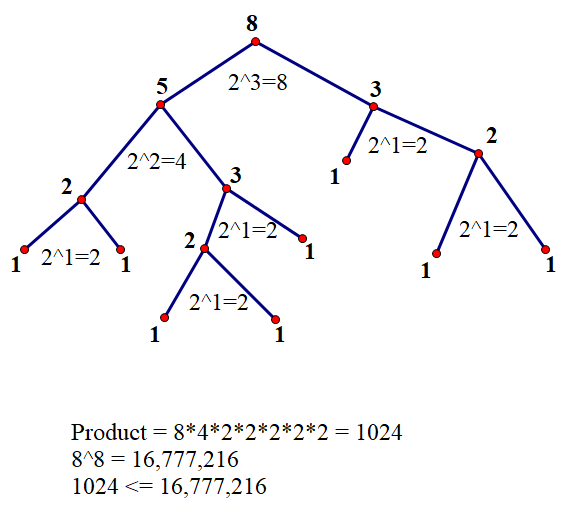
\includegraphics[scale=.75]{./Images/induction.png}\end{center}

Prove using strong induction that no matter how you split the piles, the overall product you get is less than or equal to $n^ n$.

\textbf{Hint:} When there is only one stone, you cannot split the pile, and the process stops.

\begin{solution}
Let $P(n)$ be the predicate that ``if you do this process starting with $n$ stones, the product will be less than or equal to $n^n$."

\textbf{Inductive Step:}

Let $k\geq2$ be arbitrary. Assume that for any $m$ where $1\leq m < k$, $P(m)$.  That is, if we start with any number $m$, which is fewer than $k$ stones, we will get a product less than or equal to $m^m$.

We will now prove $P(k)$.  Start with a pile of size $k$.  We will split the pile into two smaller piles of size $j$ and $k-j$, where $1\leq j\leq (k-j)<k$.  Note that $k\geq 2$, so this is valid.  Because we let $j$ be the smaller new pile, $2^j$ is the number we write down.  At this stage, we effectively repeat the entire process on both the pile with $j$ stones and the pile with $k-j$ stones, get the product from each, and multiply them together with $2^j$.  Because each pile has between $1$ and $k-j$ stones, we can apply our inductive hypothesis to each subproduct. This means:
\begin{align*}
\text{product}&\leq 2^j\cdot j^j\cdot (k-j)^{k-j} \tag{IH}\\
&=(2j)^j \cdot (k-j)^{k-j} \tag{$a^c\cdot b^c=(ab)^c$} \\
&\leq k^j \cdot k^{k-j} \tag{$j\leq k-j,$ so $2j\leq k$} \\
&=k^k.
\end{align*}
\textbf{Base Case:}

The base case is when $n=1.$ If we start with 1 stone, we don't need to split it at all to get piles with only 1 stone in it, so our product is the multiplicative identity, 1.  $1^1=1$, which is equal to our product.

\textbf{Grading Guidelines [18 points]}
\begin{gwguidelines}
    \item{+3 argues that when you start with a pile of 1 stone, that when you split it, you don't multiply anything, leaving a product of just 1 and saying that $1\le 1^1$}
    \item{+3 assumes that for some $k\in \mathbb N,$ that for all $m$ so that $1\le m\le k$ that when you start with a pile of $m$ stones, the product you get after the splitting process is less than or equal to $m^m$}
    \item{+3 starts with a pile of $k$ stones and splits that into two piles of sizes $j$ and $j'$ so that $j+j'=k$.}
    \item{+3 applies the inductive hypothesis and gets that once you're done splitting the pile of $k$ stones, you get that the end product is less than or equal to $2^j\cdot j^j\cdot (k - j)^{(k - j)}$}
    \item{+3 argues that $2^j\cdot j^j\le k^j$}
    \item{+3 arrives at the end product being less than or equal to $k^k$.}
\end{gwguidelines}
\end{solution}


\end{document}